\subsection{System Overview}
At a core level, the program consists of three or four main modules, the simulation, the renderer, a shared area and the interface, the system is designed using an object orientated structure for the simulation, renderer and shared and makes use of inheritance to reduce code repetition and simplify the underlying structure.

\paragraph{}
The main objects, render and simulation, are run on different threads, this allows the interface to remain responsive even when their is a heavy load on the simulation thread.

\paragraph{}
The shared area inherits the methods in the base class as virtual functions, these consist of set and get functions which will set and return either the control structure or a pointer container, when a pointer container is set, old data is deleted and it creates a copy of the new data to a new pointer. While it is identical, it is a whole new set of data in order to preserve thread-safety. The shared area makes use of polymorphism to modify the functions in the shared area to include mutual exclusion object

\paragraph{}
In order to simplify the management of the bodies objects and remove the automatic out of scope destruction, the objects are allocated using dynamic allocation, the disadvantage of this is that the memory must be kept under check and properly deallocated when it is no longer required. The system that is in place has been verified to delete bodies correctly and does not present any memory leaks.

\paragraph{}
The simulation thread is synchronised to the generally much slower render thread by the use of a condition variable, this interfaces to a mutex object inside the simulation main function and will pause the thread until it is unlocked by a call to the condition variable in the shared area. This effectively locks the iterations to the frame rate one to one unless the iterations per frame is more than 1. While this will result in variance should the frame rate drop below 60 frames per second, this is very unlikely because of how simplistic the graphics are, the simulation will be far slower than the rendering at any body count required to slow down the rendering even on low end and integrated GPUs.

\paragraph{}
The simulation itself makes use of a simplistic brute force method for the simulation. This calculates the forces between every single body in the scenario, this causes the time complexity of the simulation to be $O(n^2)$, the result of this is a dramatic increase in computational complexity with each body added to the simulation. The benefit of this approach is that it is by far the most accurate, as every force is calculated, something like the Barnes-Hut algorithm is less accurate, as it further approximates large clusters of bodies considering them as one large mass in a weighted mean, however this brings more advantages in terms of computation, reducing the time complexity to $O(nlogn)$.

\paragraph{}
In order to improve long term stability and general accuracy of the approximation, leapfrog integration is used, standard euler integration results in a massive deviation from initial system energies due to an accumulation of errors, this results in velocity being calculated at half time steps, while position and acceleration are calculated together. This results in a much greater stability of the simulation in both short term and long term. It also allows for the simulation to be reversed.

\paragraph{}
All forces are calculated directly as acceleration, each relationship calculated adds extra acceleration to the bodies in the $x$ and $y$ components respectively, half period velocity change and position are calculated in individual body objects directly.

\paragraph{}
The render module is relatively basic, containing functions for rendering individual bodies and the whole scene as a whole (Every body). The render class also contains a method for the creation of superstructures, a large collection of bodies all orbiting around a single point.

\paragraph{}
The interface itself is significantly less structured, as the program has to interface several different programming paradigms, including object orientated, standard procedural and event driven programming methodologies in the form of callback functions that must be set at program initialization. GLFW callbacks are passed through to AntTweakBar to allow it to access the input. The GLFW callbacks are also used for control of the camera and selection of bodies. Due to the way these callbacks work (Function Pointers), it is not directly possible to have them part of a class.

\paragraph{}
The GUI for the program was intentionally kept basic, none of the windows link together and they are all managed by the facilities of the AntTweakBar library.

\paragraph{}
Worth noting is that the AntTweakBar library is no longer maintained by the developer, the source for this library required a slight modification in order to work with the newest version of GLFW, namely when it comes to handling of inputs as the names of some decelerations have changed. The binary would need to be recompiled for this library, the modified source would likely be distributed with the source code package for the program itself, the original developer provided build systems for different operating systems so as long as dependencies are satisfied, building the modified library is straightforward. (This is not of concern to the primary user.)

\paragraph{}
Some alternative GUI packages do exist and they are actively developed, however they tend to be a lot more custom and are not as simple to set up. However having better integration into the program and an active developer community for support may outweigh this disadvantage. It would also allow for more comprehensive UI which could be far more usable and easier to add extensions to.
\pagebreak

\subsection{Algorithm Design}
\subsubsection{Calculation of All Acceleration Relationships}
This algorithms was initially extremely complex in the original specification, however after further review, it was realised that the majority of the code that was present was very redundant and only served as a memory hog. Originally the force was calculated, populated into the body objects and then acceleration was calculated on the body objects themselves.

\paragraph{}
The new code is far simpler, for starters, the force is no longer stored on the body objects, instead the force is calculated for the relationship and then it is converted to acceleration and applied to both bodies in the same method, because acceleration is still a vector quantity it can be added up in the same way that force is.

\paragraph{}
Boiling it down, this algorithm is simply a double for loop, however it makes use of the outer for loop to offset the inner for loop, effectively 'cutting-off' one half of a 'matrix'. (Including the central diagonal.) The benefit of this method is that there is no requirement to store the force in an actual matrix array, which saves on a large amount of memory. (Memory usage of a 2D array is $n^2$, which is excessive.)

\paragraph{}
The outer and inner variables are used to iterate through the body storage container, which contains pointers to the body objects. These pointers are passed to the single pair calculation method which populates both of the bodies with the acceleration produced by that relationship. Going through the double for loop will populate all of the bodies in the scenario with forces created by every other body.

\paragraph{Pseudocode}
\begin{algorithmic}[1]
\FOR{$Body_A \leftarrow 0$ \TO Bodies} 
  \FOR{$Body_B \leftarrow (Body_A+1)$ \TO Bodies}
    \STATE $Acceleration(Body_A,Body_B)$
  \ENDFOR
\ENDFOR
\end{algorithmic}

\paragraph{}
For 5 bodies, This produces iteration in order. \\
$0-1$, $0-2$, $0-3$, $0-4$, $1-2$, $1-3$, $1-4$, $2-3$, $2-4$, $3-4$ \\
No extra conditionals are required to check that $x \neq y$, Improving performance.

\pagebreak

The following is code for the above algorithm and for calculation of single relationships.
\begin{lstlisting}[language=c++]
  void simulation::calcAcceleration(body* bA, body* bB) {
    // Calculate and store distances for calculation
    double dX = getComponentDistance(bA, bB, 0);
    double dY = getComponentDistance(bA, bB, 1);
    double dV = getVectorDistance(dX, dY);

    // F=GmM/(r^3) - Pre-component force
    double fP = -(lControl.UGC * bA->m * bB->m) / std::pow(dV,3);
    // Component Forces
    double fX = fP * dX;
    double fY = fP * dY;

    // a=F/m - Set acceleration to bodies
    // Body A
    bA->aX +=  fX / bA->m;
    bA->aY +=  fY / bA->m;
    // Body B
    bB->aX += -fX / bB->m;
    bB->aY += -fY / bB->m;
  }   
  
  void simulation::calcAllAcceleration(void) {
  resetAllAcceleration(); // Set all accelerations to 0;
    for(unsigned int x = 0; x < bodies.size(); x++) {
      // Evaluate bottom left of calculation matrix
      for(unsigned int y = x+1; y < bodies.size(); y++) {
        // Same body relationships do not occur
        calcAcceleration(bodies[x], bodies[y]);
      }
    } 
  }
\end{lstlisting}

\subsubsection{Leapfrog Integration}
Leapfrog integration is the core to the stability and time-realisability functionality of the simulation. At a basic level, leapfrog integration in simply a rearrangement of the order in which Acceleration, Velocity and Position are calculated.

\paragraph{}
The Euler approach is what the majority of basic physics problems will end up using, generally because they are only asking for a single 'iteration' in order to find a solution. Euler integration makes use of a linear calculation flow of $a\rightarrow v\rightarrow r$. The issue with this is that it results in an accumulation of errors when a object cannot fit a fixed time step of movement around a curve, resulting it its path becoming larger and appearing to increase in total energy.

\paragraph{}
Leapfrog integration instead calculates velocity at a half-time step offset to acceleration and velocity, producing a calculation flow of $v_\frac{1}{2}\rightarrow r\rightarrow a\rightarrow v_\frac{1}{2}$. The velocity change in a single iteration will make use of two different accelerations, based on the change in position of all bodies. Leapfrog integration is considered to be a second order method of integration, which is the main reason for improvement over Euler integration.

\paragraph{}
The algorithm that I have implemented includes collisions and a check to ensure that none of the bodies are 'breaking the laws of physics' by leaving the simulation bounds (Very unlikely) or travelling faster than the speed of light.

\paragraph{Pseudocode}
\begin{algorithmic}[1]
\STATE $LawsOfPhyiscs$
\STATE $Velocity \times \frac{1}{2}$
\STATE $Position$
\IF{$Collide = TRUE$}
  \STATE $Collisions$
\ENDIF
\STATE $Acceleration$
\STATE $Velocity \times \frac{1}{2}$
\end{algorithmic}

\paragraph{}
The following is the code for the iteration function that is called by the main sim loop.
\begin{lstlisting}[language=c++]
  void simulation::iteration(void) {
    // Check laws of physics
    lawsOfPhysicsCheck();
    // 1/2 Velocity
    calcAllHalfVelocity();
    // Position
    calcAllPosition();
    // Collisions
    if(lControl.collide)
      calcAllCollisions();
    // Acceleration
    calcAllAcceleration();
    // 1/2 Velocity
    calcAllHalfVelocity();
  }
\end{lstlisting}

\pagebreak

\subsubsection{Mutex Locks on Shared Data}
The concept of mutual exclusion locks is relatively straightforward, a thread can lock a mutex object in executing code, if another thread attempts to execute the same code, it will reach the mutex lock code and find that the mutex is already locked, signifying that another thread is accessing a particular piece of data.

\paragraph{}
The benefit of this is that it is able to prevent simultaneous access to data in a program, this is important as simultaneous access can cause many issues when it comes to the integrity of data and the correct execution of the program. Should data be written to at the same time as writing the final read data will be garbled and could cause undefined behaviour in a program.

\paragraph{}
Originally, the code made use of a large number of mutex locks because data access in the shared area was fragmented, however the final implemented design makes use of only two mutex objects, one for the body pointer storage and one for the complete control store, while this does result in potential slow downs, the likely hood of both threads accessing data from the shared area itself it relatively unlikely.

\paragraph{}
An attempt to lock a mutex object that is already locked will result in the program waiting for the mutex to unlock until continuing. This can cause some issues if for some reason a mutex is not unlocked, such as an exception causing a thread to crash, causing deadlocks in a program that do not recover.

\paragraph{}
The inclusion of mutex objects in code is very straightforward as they are provided by the C++ STL, the most straightforward way of using them is to call the $lock$ and $unlock$ methods. However this does mean that the mutex will remain locked until unlock is explicitly called. In order to deal with this problem and simplify the programming, another feature of STL is used known as \textit{lock\_guard}. A lock\_guard will cause the object to automatically unlock when the lock\_guard object goes out of scope, solving the issue of potential deadlocks in the case of exceptions due to locked mutex objects.

\paragraph{}
It is also worth noting that the mutex code that is implemented as polymorphic method overrides over the base scenario class, while the function is still effectively the same, mutex is required in the shared class in order to prevent simultaneous access.

\paragraph{Pseudocode}
\begin{algorithmic}[1]
\STATE $Mutex.lock()$ \COMMENT{Attempt to lock mutex immediately}
\STATE $Access~Data$ \COMMENT{Read/Write}
\STATE $Mutex.unlock()$ \COMMENT{Mutex unlocks when out of scope}
\end{algorithmic}

\paragraph{}
The following is a sample of overridden methods in the shared class, the provided example contains a function that effectively reads the body pointer store and creates a full and unlinked copy, all the pointers are to new but identical body objects (dynamic allocation). The other is essentially a write operation, where the old bodies are all deleted and the new bodies are assigned from a passed container. (Copies are produced.)

\begin{lstlisting}[language=c++]
// Read Operation
std::vector<body*> shared::getBodies(void) {
  // Lock access to body store
  std::lock_guard<std::mutex> lock(bodyLock);
  std::vector<body*> r_bodies;

  r_bodies.reserve(bodies.size()); // Reserve space to create copy

  for(unsigned int i = 0; i < bodies.size(); i++) {
    r_bodies.push_back(new body(bodies[i])); // Adds to 'bodies' (Scenario Local)
  }

  return r_bodies;
}

// Write Operation
void shared::updateBodies(std::vector<body*> p_bodies) {
  // Must create a copy of objects at pointers, not just copy pointers
  // Lock access to body store
  std::lock_guard<std::mutex> lock(bodyLock);
  deleteAllBodies(); // Flush current body storage allocation
  bodies.reserve(p_bodies.size()); // Reserve space to create copy

  for(unsigned int i = 0; i < p_bodies.size(); i++) {
    addBody(new body(p_bodies[i])); // Adds to 'bodies' (Scenario Local)
  }
}
\end{lstlisting}

\paragraph{}
Without the mutex code, the read and write operation could end up being executed on two separate threads at the same time causing a large number of potential issues for the data received by the write operation, especially as it is dealing with pointers, this would likely cause pointers to be completely garbled and cause segmentation faults in the execution where illegal memory access has occurred.

\subsubsection{Calculation of Collisions}
The calculation of collisions is probably the second most computationally intensive algorithm in the program second to the primary calculation of forces. This code makes use of the same offset double for loop used in the acceleration calculation code, resulting in an effective time order complexity of $O(n^2)$ once again.

\paragraph{}
Collisions can be disabled by the user however in order to either improve performance or simply satisfy a requirement that they have for the simulation that they are carrying out. 

\paragraph{}
The collision detection works by calculating the vector distance between two bodies and checking to see if it is smaller than the sum of the radius of the two bodies, if it is, the bodies are effectively inside of each other and are therefore colliding. The collision itself is calculated as a perfectly inelastic collision, while this is not the most realistic the calculation of an inelastic collision would require more complex simulation and does not well serve the intended use of the program. 

\paragraph{}
The total mass of the two bodies in question is simply the sum of the masses, the new size of the body is defined as the sum of the areas, so the radius of the bodies is converted to area and then back to radius. The new position and velocity are slightly more complex, the position is calculated based on a weighted mean, this is a mean that includes the mass of the bodies, calculating a new position for the body which is proportional to the mass of the objects that collided.

\paragraph{}
The velocity is calculated from the sum of the momentum of the two bodies divided by the new total mass of the bodies, because it is a vector quantity it can still be performed on the x and y components as with any other variable.

\paragraph{}
If either body in the collision is fixed, the final resultant body will also be fixed.

\paragraph{}
All of the changes are by default applied to \textit{bodyA}, while \textit{bodyB} is deleted from the simulation.

\pagebreak

\paragraph{Pseudocode}
\begin{algorithmic}[1]
\FOR{$Body_A \leftarrow 1$ \TO Bodies} 
  \FOR{$Body_B \leftarrow (Body_A+1)$ \TO Bodies}
    \STATE $d_v \leftarrow getVectorDistance()$
    \IF{$d_v < r_{Body_A}+r_{Body_B}$}
      \STATE $COLLISION$
    \ENDIF
  \ENDFOR
\ENDFOR
\end{algorithmic}

\begin{lstlisting}[language=c++]
void simulation::calcAllCollisions(void) {
  for (unsigned int bA = 0; bA < bodies.size(); bA++) {
    for (unsigned int bB = bA+1; bB < bodies.size(); bB++) {
      double dX = getComponentDistance(bodies[bA], bodies[bB], 0);
      double dY = getComponentDistance(bodies[bA], bodies[bB], 1);
      double dV = getVectorDistance(xDist, yDist);

      // TODO: Implement this as an overloaded operator?
      if(dV < bodies[bA]->r+bodies[bB]->r) {
        // Body A Becomes New Body
        // Add Together Areas
        bodies[bA]->r = sqrt(pow(bodies[bA]->r,2)+pow(bodies[bB]->r,2));

        // Add Together Masses
        double totalMass = bodies[bA]->m + bodies[bB]->m;

        // Get Weighted Mean Position XY
        bodies[bA]->pX = ((bodies[bA]->pX*bodies[bA]->m) + (bodies[bB]->pX*bodies[bB]->m)) / totalMass;
        bodies[bA]->pY = ((bodies[bA]->pY*bodies[bA]->m) + (bodies[bB]->pY*bodies[bB]->m)) / totalMass;

        // Calculate New Velocity through Inelastic Collision (mv+Mv)/(m+M) = v XY
        bodies[bA]->vX = ((bodies[bA]->calcMomentum(0)) + bodies[bB]->calcMomentum(0)) / totalMass;
        bodies[bA]->vY = ((bodies[bA]->calcMomentum(1)) + bodies[bB]->calcMomentum(1)) / totalMass;

        // If either body is originally fixed, the resulting body should be fixed.
        if(bodies[bA]->fixed | bodies[bB]->fixed) bodies[bA]->fixed = true;
        // Get average of colours of both bodies - weighted mean.
        for(int c = 0; c < 3; c++) {
          bodies[bA]->color[c] = ((bodies[bA]->color[c]*bodies[bA]->m) + (bodies[bB]->color[c]*bodies[bB]->m)) / totalMass;
        }
        // Set new mass
        bodies[bA]->m = totalMass;
        // Delete Body B
        delBody(bB);
      }
    }
  }
}
\end{lstlisting}

\subsubsection{Creation of Superstructure}
The creation of a superstructure was originally just designed for testing purposes, however the user was extremely happy with the results that it was producing so it was left in and made a feature in the final program.

\paragraph{}
It makes it very easy to quickly add a large number of very organised bodies into the simulation. The algorithm makes use of pseudo-random number generation to get a relatively random distribution of bodies in the system, to start with a central body is added, then a loop adds in the number of outer bodies that are specified.

\paragraph{}
The position of the bodies is calculated using the random number provided, if the number is not greater (or smaller than the negative of it.) than the spacing set, the random number is recalculated. (The range is 0 to $2r$, when generated the radius is subtracted from it to create a positive and negative distribution. Through the use of trigonometric functions, the random number is used for both the $x$ and $y$ coordinates of the body, the trigonometric functions transform the points mapping them into to a filled circle. The random number generator is capable of generating random floating point variables, not just integers.

\paragraph{}
The distance is then calculated of the outer body to the central body and it is given circular orbital velocity around the central body. The body is then added to the scenario with all of the previously calculated values passed as parameters.

\paragraph{Pseudocode}
\begin{algorithmic}[1]\STATE $tempRand \leftarrow random(0, 200)$
\STATE $Create~central~body$
\FOR{$body \leftarrow 0$ \TO $bodies$}
  \STATE $tempRand \leftarrow random(0, 200)$
  \STATE $Calculate~position$
  \STATE $Calculate~orbital~velocity$ 
  \STATE $Create~outer~body$
\ENDFOR
\end{algorithmic}
\pagebreak
\begin{lstlisting}[language=c++]
void render::createSuperstructure(int p_soBodies, double p_cMass, double p_oMass, double p_cRadius, double p_oRadius, double p_cPosX, double p_cPosY, double p_cVelX, double p_cVelY, double p_coSpacing, double p_sRadius, float p_color[3]) {
  // Create a Pseudo-random circular distribution of bodies around a central body.

  // Use Mersenne Twister for RNE within range.
  std::uniform_real_distribution<> pos(0, p_sRadius*2);
   // Use random device for seed value
  std::random_device r;
  std::mt19937 gen(r());
  //std::mt19937 gen; // Use for desktop valgrind - random_device causes segfault

  // Temporary Variables
  double tempRand, tempCirX, tempCirY, tempDist, tempVelX, tempVelY;
  // Add Central Body
  addBody(new body(p_cMass, p_cRadius, p_cPosX, p_cPosY, p_cVelX, p_cVelY, p_color));
  //int bodyOffset = bodyStore.size() - 1;
  for(int bIDC = 0; bIDC < p_soBodies; bIDC++) {
    // Ensure that bodies are not too close to center.
    do {
      tempRand = pos(gen) - p_sRadius;
    } while((tempRand < p_coSpacing) & (tempRand > -p_coSpacing));
    // Map to Circle
    tempCirX = p_cPosX+(tempRand * std::cos(2 * M_PI * tempRand));
    tempCirY = p_cPosY+(tempRand * std::sin(2 * M_PI * tempRand));

    // Calculate Distance to Body
    tempDist = std::sqrt(std::pow(p_cPosX-tempCirX,2) + std::pow(p_cPosY-tempCirY,2));

    // Calc Velocity
    tempVelX = copysign(std::sqrt((lControl.UGC*(p_cMass+p_oMass)) / std::pow(tempDist,3)) * (tempCirY-p_cPosY), (tempCirY-p_cPosY)) + p_cVelX;
    tempVelY = copysign(std::sqrt((lControl.UGC*(p_cMass+p_oMass)) / std::pow(tempDist,3)) * (tempCirX-p_cPosX), -(tempCirX-p_cPosX)) + p_cVelY;

    addBody(new body(p_oMass, p_oRadius, tempCirX, tempCirY, tempVelX, tempVelY, p_color));
  }
}
\end{lstlisting}

\pagebreak

\subsubsection{Update UI / Update Body}
The interface was one of the more difficult pieces of code to get working as intended due to the mismatch of different programming styles and the need to maintain multiple sources of data that would be affecting the render. In order to get around the issue a compromise was made in the form of requiring the simulation to be paused before the user is able to make any change to the simulation.

\paragraph{}
In order to have a safe environment in which the data can be modified by the user, the interface includes its own pointer to a body object, this pointer does not directly point to a body object inside of the scenario container. Instead, a new body is created as a copy of the selected one from the scenario container.

\paragraph{}
On every update of the UI, the active body will be deleted and refreshed, this is to make certain that should bodies end up being deleted by the simulation due to collisions, the currently selected body does not end up referencing a body that no longer exists.

\paragraph{}
In the event that no bodies are actually present in the simulation and the body count is equal to 0, the updateUI function will populate the active body pointer with effectively a null body, this body does not exist in the scenario, but it provides somewhere for the UI variables to point to.

\paragraph{}
When the simulation is paused, updateBody is called instead of updateUI, this function takes the current active body and uses the updateBody method in the scenario class to update the instance of the body in the render scenario with the modified data, this allows for a interactive system for the modification of the bodies as the rendering continues even when the simulation is paused.

\paragraph{}
When the simulation is paused, updates are sent from the render scenario to the shared scenario, which the simulation takes while it is paused. When the simulation is not paused, it sends updates the shared area that the render scenario takes.



\begin{sidewaysfigure}
\subsection{Function Listing}
  \subsubsection{Main}
  \centering  
  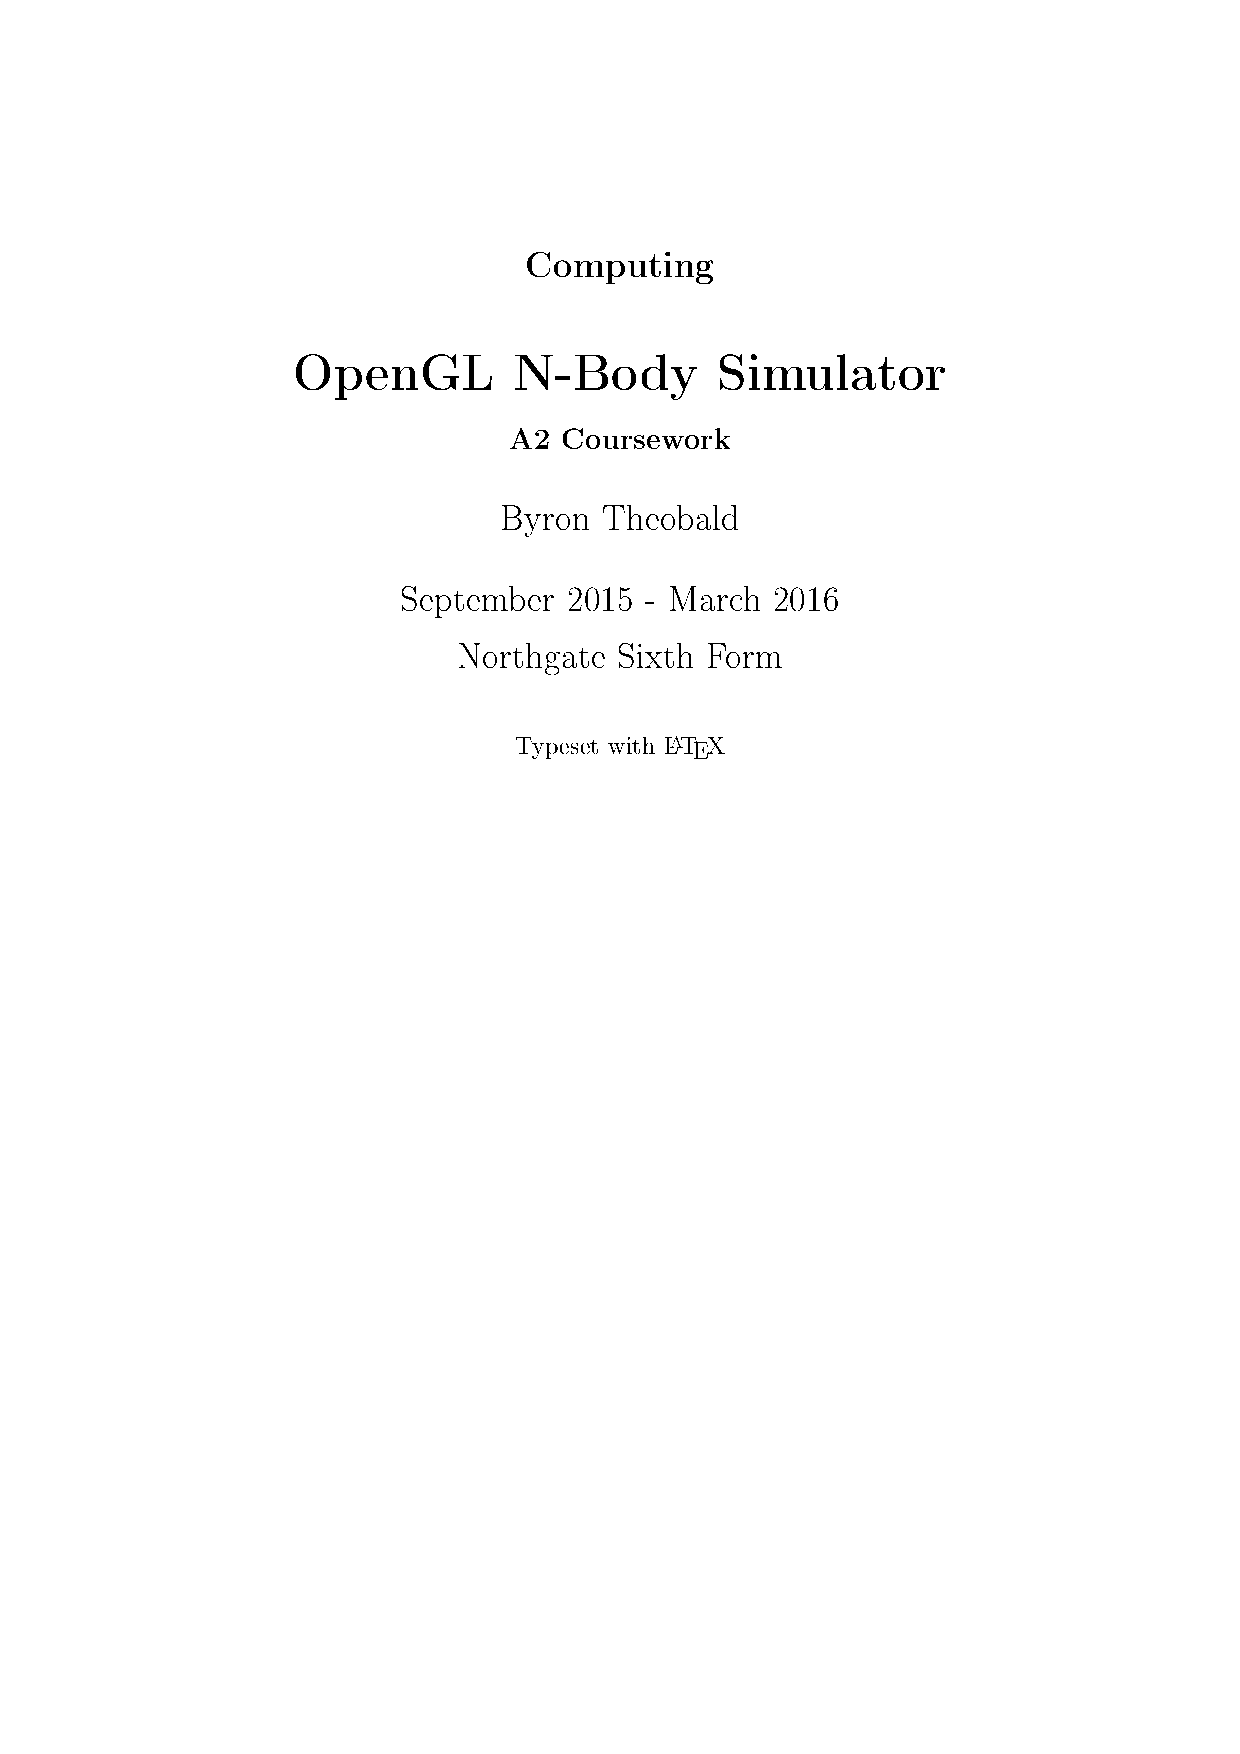
\includegraphics[width=\textwidth]{img/functions/main.png}
\end{sidewaysfigure}

\begin{sidewaysfigure}
  \subsubsection{Body}
  \centering  
  \includegraphics[width=\textwidth]{img/functions/body.png}
\end{sidewaysfigure}

\begin{sidewaysfigure}
  \subsubsection{Scenario}
  \centering  
  \includegraphics[width=\textwidth]{img/functions/scenario.png}
\end{sidewaysfigure}

\begin{sidewaysfigure}
  \subsubsection{Render}
  \centering  
  \includegraphics[width=\textwidth]{img/functions/render.png}
\end{sidewaysfigure}

\begin{sidewaysfigure}
  \subsubsection{Simulation}
  \centering  
  \includegraphics[width=\textwidth]{img/functions/simulation.png}
\end{sidewaysfigure}

\begin{sidewaysfigure}
  \subsubsection{Shared}
  \centering  
  \includegraphics[width=\textwidth]{img/functions/shared.png}
\end{sidewaysfigure}

\begin{sidewaysfigure}
  \subsubsection{UI}
  \centering  
  \includegraphics[width=\textwidth]{img/functions/ui.png}
\end{sidewaysfigure}

\begin{sidewaysfigure}
  \centering  
  \includegraphics[width=\textwidth]{img/functions/ui2.png}
\end{sidewaysfigure}

\subsection{Variable Listing}
\begin{figure}[H]
   \centering
   \includegraphics[page=1, width=\textwidth]{../varlist.pdf} 
\end{figure}

\begin{figure}[H]
   \centering
   \includegraphics[page=2, width=\textwidth]{../varlist.pdf} 
\end{figure}

\begin{figure}[H]
   \centering
   \includegraphics[page=3, width=\textwidth]{../varlist.pdf} 
\end{figure}